% !Mode:: "TeX:UTF-8"% !TEX TS-program = xelatex
% !TEX encoding = UTF-8 Unicode
% !Mode:: "TeX:UTF-8"

%+++++++++++++++++++++++++++++++++++++++++++++++++++++++++++++++++++++++++++++
% This is a sample article script. All rights reserved.
% Author: qianhui@zju.edu.cn
%+++++++++++++++++++++++++++++++++++++++++++++++++++++++++++++++++++++++++++++
\documentclass[a4paper,twoside,AutoFakeBold]{article}
% \usepackage{optreport}
\usepackage{./optreport}

%+++++++++++++++++++++++++++++++++++++++++++++++++++++++++++++++++++++++++++++
% Some packages for this sample.
%+++++++++++++++++++++++++++++++++++++++++++++++++++++++++++++++++++++++++++++
\usepackage{comment}	% Package for comment useless document
\usepackage{bm}			% Package for Bold-math symbol
\usepackage{mathrsfs}	% Package for RSFS fonts in maths
\usepackage{listings}	% Package for Listing code
\usepackage{enumerate}	% Package for enumerate
\usepackage{pdfrender}
\usepackage{subcaption}
\usepackage{multirow}
\usepackage{booktabs}
\usepackage{bbm}
\usepackage{bbding}
\usepackage{mathtools}
\usepackage{graphicx}
\usepackage{float}
\usepackage{epstopdf}
\usepackage{lipsum}
\usepackage{metalogo}

%+++++++++++++++++++++++++++++++++++++++++++++++++++++++++++++++++++++++++++++
% Title, Authors, Reprot Time.
%+++++++++++++++++++++++++++++++++++++++++++++++++++++++++++++++++++++++++++++
\serialnum{2020-3-109315041}

\rptname{A Fast Iterative Shrinkage-Thresholding Algorithm for Linear Inverse Problems}

\rptauthora{李文耀}{323101xxxx} %作者1和学号
\rptauthorb{施兴睿}{3230102392} %作者2和学号
% \rptauthorc{张三丰}{109315043} %作者3和学号
\reporttime{2025}{12}

% -------------------------------------------------
% for english version.
% -------------------------------------------------
\rptcontentsname{Contents}
\renewcommand{\abstractname}{{\xiaosan Abstract}}
\def\bibetal{et al.}
\def\biband{and}
\makeatletter
\renewcommand*{\ALG@name}{{\xiaosi Algorithm.~}}
\makeatother
\theoremstyle{definition}
\newtheorem{defn2}{{Definition}}
\newtheorem{corr2}{{Corrollary}}
\newtheorem{thrm2}{{Theorem}}
\newtheorem{lema2}{{Lemma}}
\newtheorem{exmp2}{{Example}}
\newtheorem{remark2}{{Remark}}
\renewcommand*{\proofname}{{\heiti Proof.~}}
\renewcommand{\figurename}{Fig.~}
\renewcommand{\tablename}{Tab.~}
\renewcommand{\refname}{Reference}
% -------------------------------------------------

%+++++++++++++++++++++++++++++++++++++++++++++++++++++++++++++++++++++++++++++
% Document.
%+++++++++++++++++++++++++++++++++++++++++++++++++++++++++++++++++++++++++++++
\begin{document}
\pagenumbering{gobble}

%-----------------------------------------------------------------------------
%  Title Page
%-----------------------------------------------------------------------------
\maketitle
\thispagestyle{empty} \cleardoublepage

%-----------------------------------------------------------------------------
%  Table of Content
%-----------------------------------------------------------------------------
\rptcontent \thispagestyle{empty} \cleardoublepage

%-----------------------------------------------------------------------------
%  Abstract
%-----------------------------------------------------------------------------
\begin{abstract}\kaiti \xiaosi

本文针对信号与图像处理中的线性逆问题,研究了一类基于迭代收缩阈值(ISTA)的求解算法。传统ISTA方法结构简单、易于实现,适用于大规模甚至稠密矩阵问题,但其收敛速度较慢,仅具有次线性全局收敛速率 $O(1/k)$,限制了在实际高维问题中的应用效率。为此,论文作者提出了一种快速迭代收缩阈值算法(FISTA)。该算法在保留ISTA计算简洁性的基础上,通过引入一个由历史迭代点精心构造的辅助更新项,显著提升了收敛性能。理论分析表明,FISTA 在目标函数值意义下具有 $O(1/k^2)$ 的全局收敛速率,较传统 ISTA 有了质的飞跃。此外,论文还将FISTA推广至更一般的非光滑复合优化问题,即目标函数包含光滑凸项与非光滑凸正则项。数值实验以基于小波正则化的图像去模糊为例,对比了ISTA、FISTA 以及同期提出的 TWIST 算法。实验结果表明,FISTA 在恢复质量和收敛速度上均显著优于 ISTA,且往往在迭代次数上领先数个数量级,验证了其实际有效性。

\end{abstract}
\cleardoublepage

%-----------------------------------------------------------------------------
%  Sections
%-----------------------------------------------------------------------------
\pagenumbering{arabic}\songti\xiaosi
%-----------------------
%
%-----------------------
\section{Introduction}

\subsection{Problem Background}

线性逆问题广泛存在于天体物理学、信号与图像处理、统计推断和光学等多个学科领域,其核心任务是从受噪声污染的观测数据中恢复原始信号或图像。在这类问题中,观测数据通常可建模为一个离散线性系统
$$
\bm{A} \bm{x} = \bm{b} + \bm{w}
$$

其中 $\bm{A} \in \mathbb{R}^{m \times n}$ 是已知的线性算子矩阵,$\bm{x} \in \mathbb{R}^n$ 是待估计的原始信号,$\bm{b} \in \mathbb{R}^m$ 是观测数据,$\bm{w} \in \mathbb{R}^m$ 是加性噪声。由于实际应用中常常存在测量误差和噪声,直接求解该线性系统往往会导致不稳定或不准确的结果。因此,如何有效地解决线性逆问题成为了一个重要的研究课题。求解问题的目标可以被形式化为一个最小二乘(least squares)与稀疏正则化相结合的优化问题:
$$
\min_x \{ \|\bm{A}\bm{x} -\bm{b}\|^2 + \lambda \|\bm{x}\|_1 \}
$$

尽管 $l_1$ 正则化问题可转化为二阶锥规划并利用内点法求解,但在大规模问题中,$\bm{A}$ 通常是稠密矩阵,导致内点法在计算和存储方面的开销过大,难以满足实际应用中的实时性需求。而在本篇论文发表时,代收缩阈值算法(Iterative Shrinkage-Thresholding Algorithm, ISTA)常被使用来求解该类问题。

具体而言,ISTA 的一般步骤为:
$$
\bm{x}_{k+1} = \mathcal{T}_{\lambda t} \left( \bm{x}_k - 2t \bm{A}^T (\bm{A}\bm{x}_k - \bm{b}) \right)
$$

其中 $t$ 是适当的步长,$\mathcal{T}_{\alpha}: \mathbb{R}^n \rightarrow \mathbb{R}^n$ 是收缩阈值算子,定义为:
$$
\mathcal{T}_{\alpha}(\bm{x})_i = (|x_i| - \alpha)_+ \cdot \text{sign}(x_i)
$$

其中 $(z)_+ = \max(z, 0)$,下标 $i$ 表示向量的第 $i$ 个分量。

然而尽管 ISTA 结构简单、易于实现,但其收敛速度较慢,通常仅具有 $O(1/k)$ 的次线性全局收敛速率,这在处理大规模实际问题时效率较低。在本篇论文发表前,就已经有研究者在数学上证明了 ISTA 生成的序列 $\{\bm{x}_k\}$ 在某些关于算子 $\bm{A}$ 的病态条件下可能具有极慢并且任意差的渐进收敛速率。因此,如何加速 ISTA 的收敛速度成为了一个重要的研究方向。本文正是在此背景下,针对 $l_1$ 正则化线性逆问题,提出了一种快速迭代收缩阈值算法(FISTA),旨在显著提升收敛效率,同时适用于更一般的非光滑复合优化问题。

\subsection{Contributions}

本文的核心贡献是提出了一种名为 FISTA(Fast Iterative Shrinkage-Thresholding Algorithm) 的新算法,该算法在保持 ISTA 计算简单性的同时,显著提高了全局收敛速度,并从理论和实验两方面验证了其优越性。具体贡献包括以下几个方面:

\begin{enumerate}
    \item 理论层面:提出快速迭代收缩阈值算法(FISTA)并完成收敛性证明。\\
        针对 ISTA 的慢收敛缺陷,本篇论文结合了 Nesterov 的加速思想与近端操作的适配性设计,构建了 FISTA 算法框架,还证明了 ISTA 的全局收敛速度为 $O(1/k)$,而 FISTA 则达到了 $O(1/k^2)$ 的全局收敛速率,显著优于 ISTA。这一改进是通过引入一个由历史迭代点精心构造的辅助更新点 $\bm{y}_k$ 实现的,该点由前两步迭代结果的线性组合生成,形式上为
        $$
        \bm{y}_{k+1} = \bm{x}_k + \frac{t_k}{t_{k+1}} (\bm{x}_k - \bm{x}_{k-1})
        $$
        其中 $t_k$ 按特定递归更新。这不仅降低了迭代次数的理论复杂度,还为算法在实际场景中的加速效果提供了数学保证。

        同时,这篇论文中给出的理论分析具有通用性,可处理包含任意凸非光滑正则项和任意光滑凸函数的目标函数,不局限于 $l_1$ 正则化和最小二乘损失,这使得 FISTA 能够广泛应用于各种实际问题。
    \item 实验层面:通过图像去模糊任务验证 FISTA 的性能优势。\\
        这篇论文通过在基于小波的图像去模糊问题上对比 ISTA、FISTA 以及当时最新的 TWIST 算法,实验表明 FISTA 在收敛速度上显著优于 ISTA,性能较 ISTA 提升数个数量级。在无噪声的简单测试图像恢复实验中,FISTA 仅用几百次迭代即可达到 ISTA 和 TWIST 需上万次迭代才能接近的精度。
\end{enumerate}

\subsection{Oganization}

\textbf{论文组织:}

\begin{itemize}
    \item 第一节:引言。\\
        这一部分系统性地阐述了研究背景与问题动机,指出了线性逆问题在多个领域的重要性,分析了传统 ISTA 方法的不足,并明确了提出 FISTA 的必要性和意义。
    \item 第二节:理论分析基础。\\
        这一张回顾了基于梯度的优化方法(如梯度下降、近端梯度等)的基础结论,为后续分析 ISTA 和 FISTA 提供工具。
    \item 第三节:ISTA 的全局收敛速率证明
        这一张专注于分析 ISTA 算法的收敛性能,通过理论证明 ISTA 的全局收敛速率上界为 $O(1/k)$,指出了潜在的改进方向,为后续 FISTA 的改进提供对比基准。
    \item 第四节:提出 FISTA 算法并分析其收敛性。\\
        这一节详细介绍了 FISTA 的算法框架,阐述了其设计思想,并通过严谨的数学证明,展示了 FISTA 在目标函数值意义下能达到 $O(1/k^2)$ 的全局收敛速率,显著优于 ISTA。
    \item 第五节:数值实验。\\
        这一节通过一系列数值实验,特别是在图像去模糊任务上的应用,验证了 FISTA 的实际性能。实验结果显示,FISTA 在收敛速度和恢复质量上均优于 ISTA 和同期提出的 TWIST,证明了其在实际问题中的有效性。
\end{itemize}

\textbf{记号使用:}

\begin{itemize}
    \item 两个向量 $\bm{x}, \bm{y} \in \mathbb{R}^n$ 的内积定义为 $\langle \bm{x}, \bm{y} \rangle = \bm{x}^T \bm{y}$。
    \item 矩阵 $\bm{A}$ 的最大特征值记为 $\lambda_{\max}(\bm{A})$。
    \item $\|\bm{x}\|$ 表示向量 $\bm{x}$ 的欧几里得范数。
    \item 矩阵 $\bm{A}$ 的谱范数定义记为 $\|\bm{A}\|$。
\end{itemize}



%-----------------------
%
%-----------------------
\section{相关工作}\label{section:related}

在本篇论文发表的前一段时间,有许多其他研究者也在致力于开发能提升ISTA性能的替代算法。与这篇论文提出的 FISTA 类似,这些方法不仅基于前一个迭代点,还依赖于先前计算的前两个或更多个迭代点来计算下一个迭代点。其中一条研究路径聚焦于改进 ISTA 本身,\citeauthor{bioucas-dias2007new} 提出的TWIST(两步迭代收缩/阈值)算法及其单调版本 \cite{bioucas-dias2007new} 在对问题数据和算法参数的某些假设下,能够收敛到形如
$$
\|\bm{A}\bm{x} - \bm{b}\|^2 + \varphi(\bm{x})
$$

的目标函数的极小值点,其中 $\varphi$ 是凸的非光滑正则项。TWIST 算法在当时已被验证在各类线性逆问题上效率均高于 ISTA。

而另一条尝试对同一类问题的 ISTA 进行加速的研究线路则是由 \cite{elad2007subspace} 提出的。该方法采用序列子空间优化技术进行研究,通过在一个仿射子空间上最小化函数来生成下一个迭代点,其中这个仿射子空间由两个或多个先前迭代点和当前梯度张成。这种方法的加速效果已在去噪应用问题的数值实验上得到证实。但是上述这两种方法 \cite{bioucas-dias2007new} 和 \cite{elad2007subspace} 都没有建立起对全局非渐进速率的理论分析。

在这篇论文投稿后,本篇论文的作者了解到 \citeauthor{nesterov2007gradient} 独立研究了一种加速梯度类方法的多步版本 \cite{nesterov2007gradient}。该方法与 FISTA 可以被证明在函数值上以 $O(1/k^2)$ 的速率收敛,但两者在概念和计算上都有所不同。首先,\cite{nesterov2007gradient} 利用过去迭代的累积历史递归构建一个近似函数序列 $\psi_k(\cdot)$ 来逼近 $F(\cdot)$,而 FISTA 则仅需要使用一个常规的投影类步骤。其次,\cite{nesterov2007gradient} 的方法需要在每次迭代中需要计算两次投影类操作,而 FISTA 每次迭代只需计算一次,在计算效率上更具优势,因此 FISTA 给出的方法相较于 \cite{nesterov2007gradient} 是完全不同的。


%-----------------------
%
%-----------------------
% \section{问题描述和常用记号}\label{section:preliminary}
% 本节主要描述处理的问题,并解释常用的记号。

% {\color{blue} 例如,分布式优化问题是一类重要的计算问题,在机器学习领域有大量的应用。分布式优化问题可以描述为如下形式。
% \begin{equation}\label{eq:formulation}
% \min_{x \in Q} \sum_{j \in \mathcal{N}} f_j(x).
% \end{equation}
% 在式(\ref{eq:formulation})中,$Q$是约束集合;$\mathcal{N}$是一个网络节点的索引集合;$f_j$是在$j$节点上的目标函数。
% }

% \lipsum[7]

%-----------------------
%
%-----------------------
\section{方法描述}\label{section:methods}
在本节中,算法可以表述如下算法~\ref{alg:thefirst}~所示。

\begin{algorithm}[h]\xiaosi
\caption{\xiaosi 计算 $y = x^n$}\label{alg:thefirst}
\begin{algorithmic} 
\REQUIRE $n \geq 0 \vee x \neq 0$
\ENSURE $y = x^n$
\STATE $y \leftarrow 1$
\IF{$n < 0$}
\STATE $X \leftarrow 1 / x$
\STATE $N \leftarrow -n$
\ELSE
\STATE $X \leftarrow x$
\STATE $N \leftarrow n$
\ENDIF
\WHILE{$N \neq 0$}
\IF{$N$ is even}
\STATE $X \leftarrow X \times X$
\STATE $N \leftarrow N / 2$
\ELSE[$N$ is odd]
\STATE $y \leftarrow y \times X$
\STATE $N \leftarrow N - 1$
\ENDIF
\ENDWHILE
\end{algorithmic}
\end{algorithm}

\lipsum[8]

\lipsum[9]

\lipsum[10]

%-----------------------
%
%-----------------------
\section{理论结果}\label{section:theory}
\lipsum[16]
\begin{defn2}[规范数]\label{defn:theone}
如果$x \in (0,1)$,则称$x$为规范数。
\end{defn2}
\begin{lema2}\label{lema:theone}
如果$x \in [0,1]$,则存在单调函数$\mathcal{G}(x)$ 有$\mathcal{G}(x) \geq f(x)$。
\end{lema2}
根据引理\ref{lema:theone}可以得到我们给出如下定理。
\begin{thrm2}\label{thrm:theone}
如果$x \in [0,1]$,则有$f(x) \geq f(y) + (x-y)^{\top} \nabla \mathcal{G}(x)$ 当且仅当 $f(\cdot)$是凸函数。
\end{thrm2}
根据定理\ref{thrm:theone}可以得到如下推论。
\begin{corr2}\label{corr:theone}
如果$x \in [0,1]$,则有$f(x)$是单调函数。
\end{corr2}
\begin{proof}
引理证明如下。
\end{proof}
\begin{exmp2}\label{corr:theone}
$f(x)= ax + b$,其中$a>0$。
\end{exmp2}

\begin{remark2}\label{remark:theone}
$f(x)$是单调函数。
\end{remark2}

\lipsum[28-29]
\subsection{收敛率相关理论结果}
\lipsum[31]
\subsubsection{光滑函数}
\lipsum[32]
\subsubsection{非光滑函数}
\lipsum[33]

\subsection{其他重要理论结果}
\lipsum[36]
\subsubsection{光滑函数}
\lipsum[34]
\subsubsection{非光滑函数}
\lipsum[35]

%-----------------------
%
%-----------------------
\section{应用意义}\label{section:application}
阐述上述理论有哪些应用,可以列举使用了上述理论的论文、专利、软硬件产品等。

\lipsum[16-24]

%-----------------------
%
%-----------------------
\section{实验}\label{section:experiment}
请描述清楚实验的基本设置,例如:用何种数据集?参数是如何设定的?实验结果数据的来源(是自己做的实验还是引自他人的结果,如果是他人完成的实验,要注明参考文献)。建议要有实验的基本分析。实验的图的例子可参考图\ref{figure_LR_curves}。

\lipsum[25-26]
\begin{figure}[ht]
	\begin{subfigure}{.48\textwidth}
		\centering
		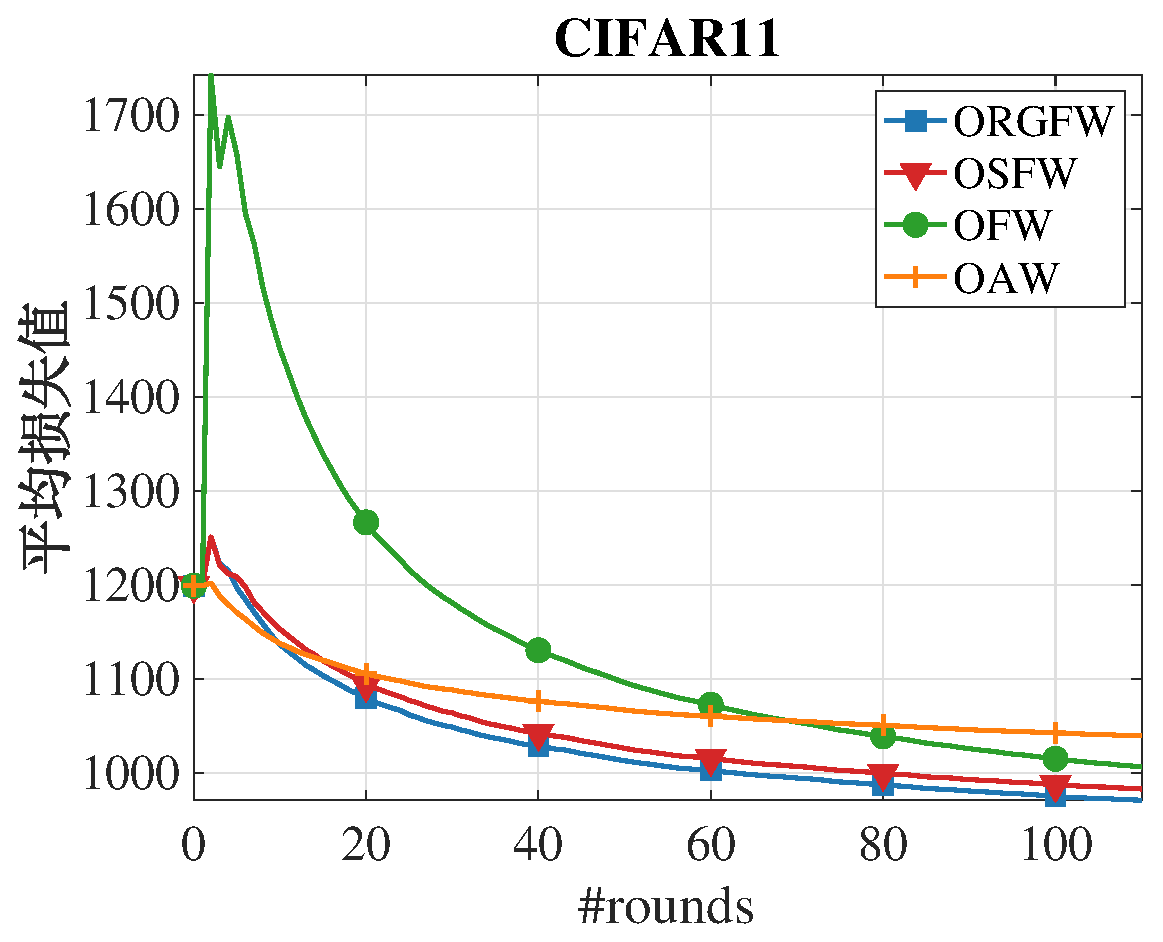
\includegraphics[width=\linewidth]{figs/CIFAR11_adv_regret}
	\end{subfigure}
	\hfill
	\begin{subfigure}{.48\textwidth}
		\centering
		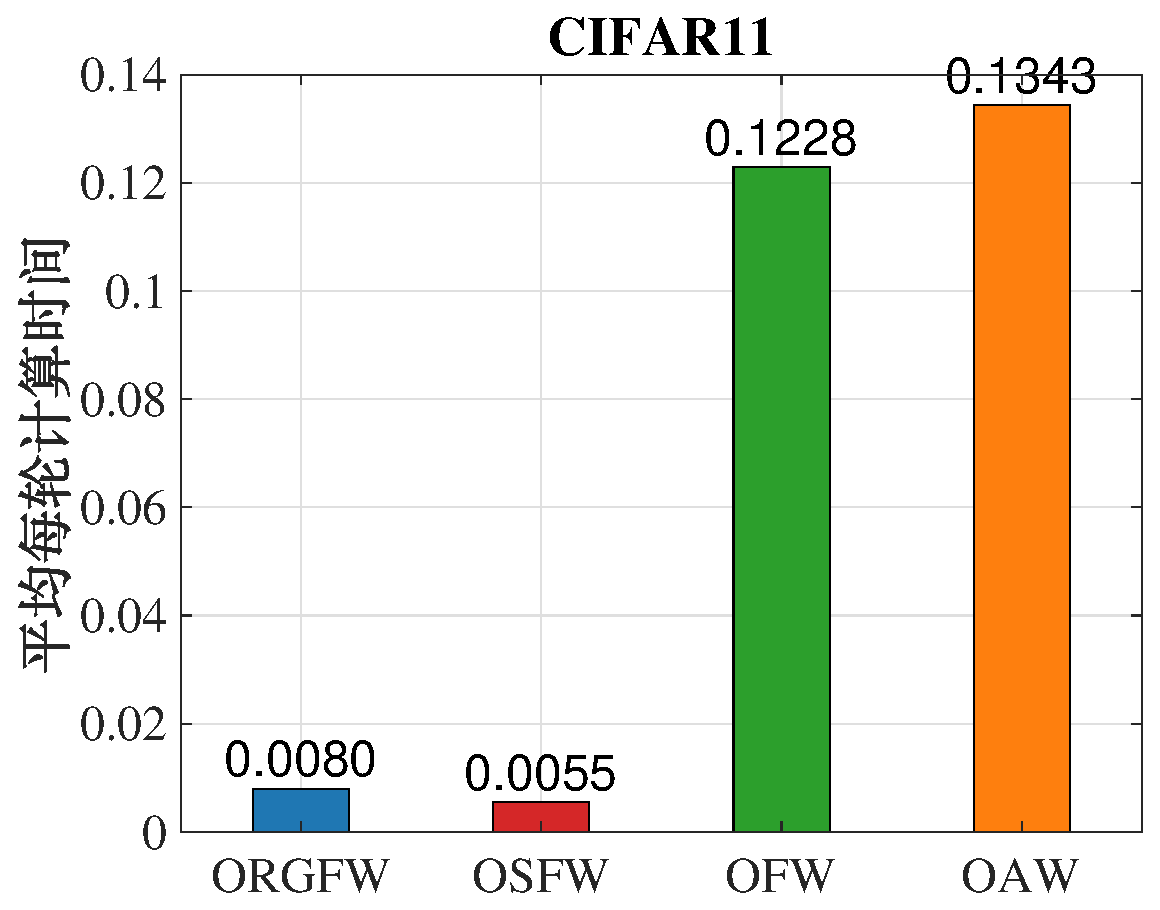
\includegraphics[width=\linewidth]{figs/CIFAR11_adv_time}
	\end{subfigure}
	\caption[在线多分类Logistic回归任务的实验结果]{
		在线多分类Logistic回归任务的实验结果。
		左边曲线图的横轴表示轮数,纵轴表示平均的损失函数值。
		右边的柱状图展示了每个算法平均每轮的计算时间。
	}
	\label{figure_LR_curves}
\end{figure}
\lipsum[27]

%-----------------------
%
%-----------------------
\section{总结}\label{section:conclusion}
\lipsum[28]


%+++++++++++++++++++++++++++++++++++++++++++++++++++++++++++++++++++++++++++++
% Bibliography
%+++++++++++++++++++++++++++++++++++++++++++++++++++++++++++++++++++++++++++++
\bibliographystyle{gbt7714-plain}
\bibliography{main}

%+++++++++++++++++++++++++++++++++++++++++++++++++++++++++++++++++++++++++++++
\end{document}
%+++++++++++++++++++++++++++++++++++++++++++++++++++++++++++++++++++++++++++++


